\chapter{Algoritmi na znakovnim nizovima}

Ovo poglavlje obrađuje efikasne algoritme
za obradu znakovnih nizova.
Mnogi se zadaci sa znakovnim nizovima mogu lako riješiti
u $O(n^2)$ vremenu, ali izazov je
naći algoritme koji rade u $O(n)$ ili $O(n \log n)$
vremenu.

\index{traženje uzorka}

Na primjer, temeljni zadatak obrade znakovnih
nizova je zadatak \key{traženja uzorka}:
zadan je znakovni niz duljine $n$ i uzorak duljine $m$,
a naš je zadatak naći pojave uzorka
u znakovnom nizu.
Na primjer, uzorak \texttt{ABC} pojavljuje se dva
puta u znakovnom nizu \texttt{ABABCBABC}.

Zadatak traženja uzorka može se lako riješiti
u $O(nm)$ vremenu algoritmom grube sile koji
provjerava sve pozicije na kojima se uzorak može
pojaviti u znakovnom nizu.
No u ovom ćemo poglavlju vidjeti da postoje
efikasniji algoritmi koji zahtijevaju samo
$O(n+m)$ vremena.

\index{znakovni niz}

\section{Terminologija znakovnih nizova}

\index{abeceda}

Kroz cijelo poglavlje pretpostavljamo da se
u znakovnim nizovima indeksira od nule.
Dakle, znakovni niz \texttt{s} duljine $n$
sastoji se od znakova
$\texttt{s}[0],\texttt{s}[1],\ldots,\texttt{s}[n-1]$.
Skup znakova koji se mogu pojaviti
u znakovnim nizovima nazivamo \key{abeceda}.
Na primjer, abeceda
$\{\texttt{A},\texttt{B},\ldots,\texttt{Z}\}$
sastoji se od velikih slova engleskog jezika.

\index{podniz znakova}

\key{Podniz znakova} je niz uzastopnih
znakova u znakovnom nizu.
Koristimo oznaku $\texttt{s}[a \ldots b]$
za podniz znakova niza \texttt{s}
koji počinje na poziciji $a$ i završava na poziciji $b$.
Znakovni niz duljine $n$ ima $n(n+1)/2$ podnizova znakova.
Na primjer, podnizovi znakova niza
\texttt{ABCD} su
\texttt{A}, \texttt{B}, \texttt{C}, \texttt{D},
\texttt{AB}, \texttt{BC}, \texttt{CD},
\texttt{ABC}, \texttt{BCD} i \texttt{ABCD}.

\index{podslijed}

\key{Podslijed} je niz
(ne nužno uzastopnih) znakova
u znakovnom nizu u njihovu izvornom redoslijedu.
Znakovni niz duljine $n$ ima $2^n-1$ podslijedova.
Na primjer, podslijedovi niza
\texttt{ABCD} su
\texttt{A}, \texttt{B}, \texttt{C}, \texttt{D},
\texttt{AB}, \texttt{AC}, \texttt{AD},
\texttt{BC}, \texttt{BD}, \texttt{CD},
\texttt{ABC}, \texttt{ABD}, \texttt{ACD},
\texttt{BCD} i \texttt{ABCD}.

\index{prefiks}
\index{sufiks}

\key{Prefiks} je podniz znakova koji počinje na početku
znakovnog niza,
a \key{sufiks} je podniz znakova koji završava na kraju
znakovnog niza.
Na primjer,
prefiksi niza \texttt{ABCD} su
\texttt{A}, \texttt{AB}, \texttt{ABC} i \texttt{ABCD},
a sufiksi niza \texttt{ABCD} su
\texttt{D}, \texttt{CD}, \texttt{BCD} i \texttt{ABCD}.

\index{rotacija}

\key{Rotaciju} možemo dobiti premještanjem
znakova znakovnog niza jednog po jednog s početka
na kraj (ili obratno).
Na primjer, rotacije niza \texttt{ABCD} su
\texttt{ABCD}, \texttt{BCDA}, \texttt{CDAB} i \texttt{DABC}.

\index{period}

\key{Period} je prefiks znakovnog niza takav da se
niz može konstruirati ponavljanjem toga perioda.
Posljednje ponavljanje može biti djelomično i sadržavati
samo prefiks perioda.
Na primjer, najkraći period niza
\texttt{ABCABCA} je \texttt{ABC}.

\index{rub}

\key{Rub} je znakovni niz koji je istodobno
i prefiks i sufiks nekog znakovnog niza.
Na primjer, rubovi niza \texttt{ABACABA}
su \texttt{A}, \texttt{ABA} i \texttt{ABACABA}.

\index{leksikografski poredak}

Znakovni nizovi uspoređuju se pomoću \key{leksikografskog poretka}
(koji odgovara abecednom poretku).
To znači da je $x<y$ ako je $x \neq y$ i $x$ je prefiks od $y$,
ili ako postoji pozicija $k$ takva da je
$x[i]=y[i]$ za $i<k$ i $x[k]<y[k]$.

\section{Struktura trie}

\index{trie}

\key{Trie} je ukorijenjeno stablo koje
održava skup znakovnih nizova.
Svaki znakovni niz u skupu pohranjen je kao
lanac znakova koji počinje u korijenu.
Ako dva znakovna niza imaju zajednički prefiks,
imaju i zajednički lanac u stablu.

Na primjer, razmotrimo sljedeći trie:

\begin{center}
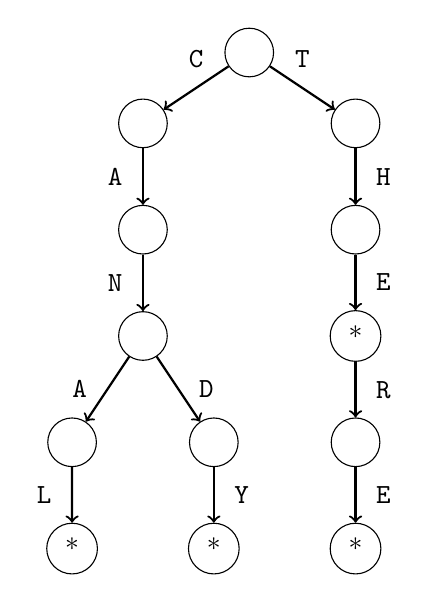
\begin{tikzpicture}[scale=0.9]
\node[draw, circle] (1) at (0,20) {$\phantom{1}$};
\node[draw, circle] (2) at (-1.5,19) {$\phantom{1}$};
\node[draw, circle] (3) at (1.5,19) {$\phantom{1}$};
\node[draw, circle] (4) at (-1.5,17.5) {$\phantom{1}$};
\node[draw, circle] (5) at (-1.5,16) {$\phantom{1}$};
\node[draw, circle] (6) at (-2.5,14.5) {$\phantom{1}$};
\node[draw, circle] (7) at (-0.5,14.5) {$\phantom{1}$};
\node[draw, circle] (8) at (-2.5,13) {*};
\node[draw, circle] (9) at (-0.5,13) {*};
\node[draw, circle] (10) at (1.5,17.5) {$\phantom{1}$};
\node[draw, circle] (11) at (1.5,16) {*};
\node[draw, circle] (12) at (1.5,14.5) {$\phantom{1}$};
\node[draw, circle] (13) at (1.5,13) {*};

\path[draw,thick,->] (1) -- node[font=\small,label=\texttt{C}] {} (2);
\path[draw,thick,->] (1) -- node[font=\small,label=\texttt{T}] {} (3);
\path[draw,thick,->] (2) -- node[font=\small,label=left:\texttt{A}] {} (4);
\path[draw,thick,->] (4) -- node[font=\small,label=left:\texttt{N}] {} (5);
\path[draw,thick,->] (5) -- node[font=\small,label=left:\texttt{A}] {} (6);
\path[draw,thick,->] (5) -- node[font=\small,label=right:\texttt{D}] {} (7);
\path[draw,thick,->] (6) -- node[font=\small,label=left:\texttt{L}] {}(8);
\path[draw,thick,->] (7) -- node[font=\small,label=right:\texttt{Y}] {} (9);
\path[draw,thick,->] (3) -- node[font=\small,label=right:\texttt{H}] {} (10);
\path[draw,thick,->] (10) -- node[font=\small,label=right:\texttt{E}] {} (11);
\path[draw,thick,->] (11) -- node[font=\small,label=right:\texttt{R}] {} (12);
\path[draw,thick,->] (12) -- node[font=\small,label=right:\texttt{E}] {} (13);
\end{tikzpicture}
\end{center}

Ovaj trie odgovara skupu
$\{\texttt{CANAL},\texttt{CANDY},\texttt{THE},\texttt{THERE}\}$.
Znak * u čvoru znači da
u tom čvoru završava neki znakovni niz iz skupa.
Takav je znak potreban jer znakovni niz
može biti prefiks drugog znakovnog niza.
Na primjer, u gornjem trieu, \texttt{THE}
je prefiks niza \texttt{THERE}.

U $O(n)$ vremenu možemo provjeriti sadrži li trie
znakovni niz duljine $n$,
jer možemo pratiti lanac koji počinje u korijenskom čvoru.
Znakovni niz duljine $n$ možemo također dodati u trie
u $O(n)$ vremenu tako da najprije pratimo lanac,
a zatim po potrebi dodamo nove čvorove u trie.

Pomoću triea možemo naći
najdulji prefiks danog znakovnog niza
takav da taj prefiks pripada skupu.
Nadalje, pohranjivanjem dodatnih informacija
u svaki čvor
možemo izračunati broj
znakovnih nizova koji pripadaju skupu i imaju
dani znakovni niz kao prefiks.

Trie možemo pohraniti u niz
\begin{lstlisting}
int trie[N][A];
\end{lstlisting}
gdje je $N$ najveći broj čvorova
(najveća ukupna duljina znakovnih nizova u skupu),
a $A$ je veličina abecede.
Čvorovi triea numerirani su
$0,1,2,\ldots$ tako da je broj korijena 0,
a $\texttt{trie}[s][c]$ je sljedeći čvor u lancu
kad se iz čvora $s$ pomaknemo koristeći znak $c$.

\section{Raspršivanje znakovnih nizova}

\index{raspršivanje}
\index{raspršivanje znakovnih nizova}

\key{Raspršivanje znakovnih nizova} tehnika je koja
nam omogućuje efikasnu provjeru jesu li dva
znakovna niza jednaka\footnote{Tehniku je
popularizirao Karp–Rabinov algoritam za traženje
uzorka \cite{kar87}.}.
Ideja raspršivanja je usporediti hash vrijednosti
znakovnih nizova umjesto njihovih pojedinih znakova.

\subsubsection*{Računanje hash vrijednosti}

\index{hash vrijednost}
\index{polinomno raspršivanje}

\key{Hash vrijednost} znakovnog niza
broj je koji se izračuna iz znakova
toga niza.
Ako su dva znakovna niza jednaka,
jednake su i njihove hash vrijednosti,
što omogućuje uspoređivanje znakovnih nizova
na temelju njihovih hash vrijednosti.

Uobičajen način implementacije raspršivanja
je \key{polinomno raspršivanje}, što znači
da je hash vrijednost znakovnog niza \texttt{s}
duljine $n$ jednaka
\[(\texttt{s}[0] A^{n-1} + \texttt{s}[1] A^{n-2} + \cdots + \texttt{s}[n-1] A^0) \bmod B  ,\]
gdje se $s[0],s[1],\ldots,s[n-1]$
interpretiraju kao kodovi znakova niza \texttt{s},
a $A$ i $B$ su unaprijed odabrane konstante.

Na primjer, kodovi znakova
niza \texttt{ALLEY} su:
\begin{center}
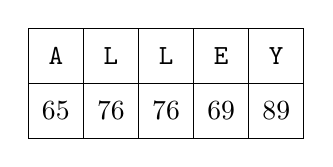
\begin{tikzpicture}[scale=0.7]
\draw (0,0) grid (5,2);

\node at (0.5, 1.5) {\texttt{A}};
\node at (1.5, 1.5) {\texttt{L}};
\node at (2.5, 1.5) {\texttt{L}};
\node at (3.5, 1.5) {\texttt{E}};
\node at (4.5, 1.5) {\texttt{Y}};

\node at (0.5, 0.5) {65};
\node at (1.5, 0.5) {76};
\node at (2.5, 0.5) {76};
\node at (3.5, 0.5) {69};
\node at (4.5, 0.5) {89};

\end{tikzpicture}
\end{center}

Dakle, ako je $A=3$ i $B=97$, hash vrijednost
niza \texttt{ALLEY} je
\[(65 \cdot 3^4 + 76 \cdot 3^3 + 76 \cdot 3^2 + 69 \cdot 3^1 + 89 \cdot 3^0) \bmod 97 = 52.\]

\subsubsection*{Predobrada}

Pomoću polinomnog raspršivanja možemo izračunati hash vrijednost bilo kojeg
podniza znakova niza \texttt{s} u $O(1)$ vremenu nakon predobrade u $O(n)$ vremenu.
Ideja je konstruirati niz \texttt{h} takav da
$\texttt{h}[k]$ sadrži hash vrijednost prefiksa $\texttt{s}[0 \ldots k]$.
Vrijednosti niza mogu se rekurzivno izračunati na sljedeći način:
\[
\begin{array}{lcl}
\texttt{h}[0] & = & \texttt{s}[0] \\
\texttt{h}[k] & = & (\texttt{h}[k-1] A + \texttt{s}[k]) \bmod B \\
\end{array}
\]
Osim toga, konstruiramo niz $\texttt{p}$
gdje je $\texttt{p}[k]=A^k \bmod B$:
\[
\begin{array}{lcl}
\texttt{p}[0] & = & 1 \\
\texttt{p}[k] & = & (\texttt{p}[k-1] A) \bmod B. \\
\end{array}
\]
Konstrukcija tih nizova traži $O(n)$ vremena.
Nakon toga hash vrijednost bilo kojeg podniza znakova
$\texttt{s}[a \ldots b]$
može se izračunati u $O(1)$ vremenu pomoću formule
\[(\texttt{h}[b]-\texttt{h}[a-1] \texttt{p}[b-a+1]) \bmod B\]
uz pretpostavku da je $a>0$.
Ako je $a=0$, hash vrijednost je jednostavno $\texttt{h}[b]$.

\subsubsection*{Uporaba hash vrijednosti}

Znakovne nizove možemo efikasno uspoređivati pomoću hash vrijednosti.
Ideja je da umjesto uspoređivanja pojedinih znakova nizova
uspoređujemo njihove hash vrijednosti.
Ako su hash vrijednosti jednake,
nizovi su \emph{vjerojatno} jednaki,
a ako su hash vrijednosti različite,
nizovi su \emph{sigurno} različiti.

Pomoću raspršivanja često možemo algoritam grube sile
učiniti efikasnim.
Kao primjer razmotrimo zadatak traženja uzorka:
zadan je znakovni niz $s$ i uzorak $p$,
a treba naći pozicije na kojima se $p$ pojavljuje u $s$.
Algoritam grube sile prolazi kroz sve pozicije
na kojima se $p$ može pojaviti i uspoređuje nizove
znak po znak.
Vremenska složenost takvog algoritma je $O(n^2)$.

Algoritam grube sile možemo učiniti efikasnijim
koristeći raspršivanje, jer algoritam uspoređuje
podnizove znakova nizova.
Uz raspršivanje svaka usporedba traži samo $O(1)$ vremena,
jer se uspoređuju samo hash vrijednosti podnizova znakova.
Rezultat je algoritam vremenske složenosti $O(n)$,
što je najbolja moguća vremenska složenost za ovaj zadatak.

Kombiniranjem raspršivanja i \emph{binarnog traženja}
moguće je i odrediti leksikografski poredak
dvaju znakovnih nizova u logaritamskom vremenu.
To možemo postići tako da binarnim traženjem izračunamo duljinu
zajedničkog prefiksa tih nizova.
Kad znamo duljinu zajedničkog prefiksa,
dovoljno je provjeriti prvi znak nakon prefiksa,
jer on određuje poredak nizova.

\subsubsection*{Kolizije i parametri}

\index{kolizija}

Očita opasnost pri uspoređivanju hash vrijednosti je
\key{kolizija}, što znači da dva znakovna niza imaju
različit sadržaj, ali jednake hash vrijednosti.
U tom slučaju algoritam koji se pouzdaje u
hash vrijednosti zaključuje da su nizovi jednaki,
iako to u stvarnosti nisu,
pa algoritam može dati netočne rezultate.

Kolizije su uvijek moguće,
jer je broj različitih znakovnih nizova veći
od broja različitih hash vrijednosti.
Međutim, vjerojatnost kolizije mala je
ako su konstante $A$ i $B$ pažljivo odabrane.
Uobičajeno je odabrati slučajne konstante
blizu $10^9$, na primjer ovako:
\[
\begin{array}{lcl}
A & = & 911382323 \\
B & = & 972663749 \\
\end{array}
\]

Uz takve konstante
pri računanju hash vrijednosti možemo koristiti
tip \texttt{long long},
jer će umnošci $AB$ i $BB$ stati u \texttt{long long}.
No je li dovoljno imati oko $10^9$ različitih hash vrijednosti?

Razmotrimo tri scenarija u kojima se raspršivanje može koristiti:

\textit{Scenarij 1:} Znakovni nizovi $x$ i $y$ uspoređuju se
međusobno.
Vjerojatnost kolizije je $1/B$ uz pretpostavku da su
sve hash vrijednosti jednako vjerojatne.

\textit{Scenarij 2:} Znakovni niz $x$ uspoređuje se s nizovima
$y_1,y_2,\ldots,y_n$.
Vjerojatnost jedne ili više kolizija je

\[1-(1-\frac{1}{B})^n.\]

\textit{Scenarij 3:} Svi parovi znakovnih nizova $x_1,x_2,\ldots,x_n$
uspoređuju se međusobno.
Vjerojatnost jedne ili više kolizija je
\[ 1 - \frac{B \cdot (B-1) \cdot (B-2) \cdots (B-n+1)}{B^n}.\]

Sljedeća tablica prikazuje vjerojatnosti kolizije
kad je $n=10^6$, a vrijednost $B$ varira:

\begin{center}
\begin{tabular}{rrrr}
konstanta $B$ & scenarij 1 & scenarij 2 & scenarij 3 \\
\hline
$10^3$ & $0.001000$ & $1.000000$ & $1.000000$ \\
$10^6$ & $0.000001$ & $0.632121$ & $1.000000$ \\
$10^9$ & $0.000000$ & $0.001000$ & $1.000000$ \\
$10^{12}$ & $0.000000$ & $0.000000$ & $0.393469$ \\
$10^{15}$ & $0.000000$ & $0.000000$ & $0.000500$ \\
$10^{18}$ & $0.000000$ & $0.000000$ & $0.000001$ \\
\end{tabular}
\end{center}

Tablica pokazuje da je u scenariju 1
vjerojatnost kolizije zanemariva
kad je $B \approx 10^9$.
U scenariju 2 kolizija je moguća, ali je
vjerojatnost još uvijek dosta mala.
U scenariju 3, međutim, situacija je posve drugačija:
kolizija će se gotovo uvijek dogoditi kad je
$B \approx 10^9$.

\index{paradoks rođendana}

Pojava iz scenarija 3 poznata je kao
\key{paradoks rođendana}: ako je $n$ ljudi
u prostoriji, vjerojatnost da \emph{neke} dvije osobe
imaju isti datum rođenja velika je i kad je $n$ prilično mali.
Kod raspršivanja je, analogno, kad se sve hash vrijednosti
uspoređuju međusobno, velika vjerojatnost da su neke dvije
hash vrijednosti jednake.

Vjerojatnost kolizije možemo smanjiti
računanjem \emph{više} hash vrijednosti
s različitim parametrima.
Malo je vjerojatno da bi kolizija nastupila
u svim hash vrijednostima istodobno.
Na primjer, dvije hash vrijednosti s parametrom
$B \approx 10^9$ odgovaraju jednoj hash
vrijednosti s parametrom $B \approx 10^{18}$,
što čini vjerojatnost kolizije vrlo malom.

Neki koriste konstante $B=2^{32}$ i $B=2^{64}$,
što je praktično jer se operacije s 32-bitnim i 64-bitnim
cijelim brojevima računaju modulo $2^{32}$ i $2^{64}$.
Međutim, to \emph{nije} dobar odabir, jer je moguće
konstruirati ulaze koji uvijek generiraju kolizije kad se
koriste konstante oblika $2^x$ \cite{pac13}.

\section{Z-algoritam}

\index{Z-algoritam}
\index{Z-niz}

\key{Z-niz} \texttt{z} znakovnog niza \texttt{s}
duljine $n$ sadrži za svaki $k=0,1,\ldots,n-1$
duljinu najduljeg podniza znakova niza \texttt{s}
koji počinje na poziciji $k$ i prefiks je niza \texttt{s}.
Dakle, $\texttt{z}[k]=p$ govori nam da je
$\texttt{s}[0 \ldots p-1]$ jednako $\texttt{s}[k \ldots k+p-1]$.
Mnogi se zadaci obrade znakovnih nizova mogu efikasno riješiti
pomoću Z-niza.

Na primjer, Z-niz niza
\texttt{ACBACDACBACBACDA} je sljedeći:

\begin{center}
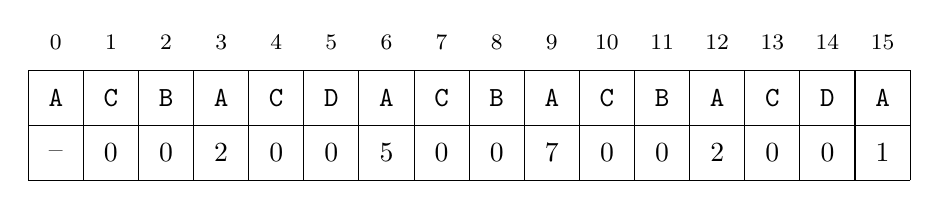
\begin{tikzpicture}[scale=0.7]
\draw (0,0) grid (16,2);

\node at (0.5, 1.5) {\texttt{A}};
\node at (1.5, 1.5) {\texttt{C}};
\node at (2.5, 1.5) {\texttt{B}};
\node at (3.5, 1.5) {\texttt{A}};
\node at (4.5, 1.5) {\texttt{C}};
\node at (5.5, 1.5) {\texttt{D}};
\node at (6.5, 1.5) {\texttt{A}};
\node at (7.5, 1.5) {\texttt{C}};
\node at (8.5, 1.5) {\texttt{B}};
\node at (9.5, 1.5) {\texttt{A}};
\node at (10.5, 1.5) {\texttt{C}};
\node at (11.5, 1.5) {\texttt{B}};
\node at (12.5, 1.5) {\texttt{A}};
\node at (13.5, 1.5) {\texttt{C}};
\node at (14.5, 1.5) {\texttt{D}};
\node at (15.5, 1.5) {\texttt{A}};

\node at (0.5, 0.5) {--};
\node at (1.5, 0.5) {0};
\node at (2.5, 0.5) {0};
\node at (3.5, 0.5) {2};
\node at (4.5, 0.5) {0};
\node at (5.5, 0.5) {0};
\node at (6.5, 0.5) {5};
\node at (7.5, 0.5) {0};
\node at (8.5, 0.5) {0};
\node at (9.5, 0.5) {7};
\node at (10.5, 0.5) {0};
\node at (11.5, 0.5) {0};
\node at (12.5, 0.5) {2};
\node at (13.5, 0.5) {0};
\node at (14.5, 0.5) {0};
\node at (15.5, 0.5) {1};

\footnotesize
\node at (0.5, 2.5) {0};
\node at (1.5, 2.5) {1};
\node at (2.5, 2.5) {2};
\node at (3.5, 2.5) {3};
\node at (4.5, 2.5) {4};
\node at (5.5, 2.5) {5};
\node at (6.5, 2.5) {6};
\node at (7.5, 2.5) {7};
\node at (8.5, 2.5) {8};
\node at (9.5, 2.5) {9};
\node at (10.5, 2.5) {10};
\node at (11.5, 2.5) {11};
\node at (12.5, 2.5) {12};
\node at (13.5, 2.5) {13};
\node at (14.5, 2.5) {14};
\node at (15.5, 2.5) {15};

\end{tikzpicture}
\end{center}

U ovom slučaju je, na primjer, $\texttt{z}[6]=5$,
jer je podniz znakova \texttt{ACBAC} duljine 5
prefiks niza \texttt{s},
ali podniz znakova \texttt{ACBACB} duljine 6
nije prefiks niza \texttt{s}.

\subsubsection*{Opis algoritma}

Slijedi opis algoritma,
zvanog \key{Z-algoritam}\footnote{Z-algoritam je
predstavljen u \cite{gus97} kao najjednostavnija poznata
metoda za traženje uzorka u linearnom vremenu, a izvorna ideja
pripisana je \cite{mai84}.},
koji efikasno konstruira Z-niz u $O(n)$ vremenu.
Algoritam računa vrijednosti Z-niza
slijeva na desno tako da istodobno koristi informacije
koje su već pohranjene u Z-nizu i uspoređuje podnizove znakova
znak po znak.

Za efikasno računanje vrijednosti Z-niza
algoritam održava interval $[x,y]$ takav da je
$\texttt{s}[x \ldots y]$ prefiks niza \texttt{s}
i da je $y$ što je veći moguće.
Budući da znamo da su $\texttt{s}[0 \ldots y-x]$
i $\texttt{s}[x \ldots y]$ jednaki,
možemo tu informaciju iskoristiti pri računanju
Z-vrijednosti za pozicije $x+1,x+2,\ldots,y$.

Na svakoj poziciji $k$ najprije
provjerimo vrijednost $\texttt{z}[k-x]$.
Ako je $k+\texttt{z}[k-x]<y$, znamo da je $\texttt{z}[k]=\texttt{z}[k-x]$.
Međutim, ako je $k+\texttt{z}[k-x] \ge y$,
$\texttt{s}[0 \ldots y-k]$ jednako je
$\texttt{s}[k \ldots y]$, pa za određivanje
vrijednosti $\texttt{z}[k]$ moramo usporediti
podnizove znakova znak po znak.
Algoritam ipak radi u $O(n)$ vremenu,
jer uspoređivanje počinjemo na pozicijama
$y-k+1$ i $y+1$.

Na primjer, konstruirajmo sljedeći Z-niz:

\begin{center}
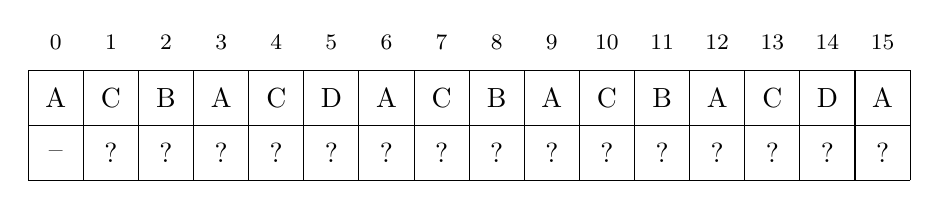
\begin{tikzpicture}[scale=0.7]
\draw (0,0) grid (16,2);

\node at (0.5, 1.5) {A};
\node at (1.5, 1.5) {C};
\node at (2.5, 1.5) {B};
\node at (3.5, 1.5) {A};
\node at (4.5, 1.5) {C};
\node at (5.5, 1.5) {D};
\node at (6.5, 1.5) {A};
\node at (7.5, 1.5) {C};
\node at (8.5, 1.5) {B};
\node at (9.5, 1.5) {A};
\node at (10.5, 1.5) {C};
\node at (11.5, 1.5) {B};
\node at (12.5, 1.5) {A};
\node at (13.5, 1.5) {C};
\node at (14.5, 1.5) {D};
\node at (15.5, 1.5) {A};

\node at (0.5, 0.5) {--};
\node at (1.5, 0.5) {?};
\node at (2.5, 0.5) {?};
\node at (3.5, 0.5) {?};
\node at (4.5, 0.5) {?};
\node at (5.5, 0.5) {?};
\node at (6.5, 0.5) {?};
\node at (7.5, 0.5) {?};
\node at (8.5, 0.5) {?};
\node at (9.5, 0.5) {?};
\node at (10.5, 0.5) {?};
\node at (11.5, 0.5) {?};
\node at (12.5, 0.5) {?};
\node at (13.5, 0.5) {?};
\node at (14.5, 0.5) {?};
\node at (15.5, 0.5) {?};

\footnotesize
\node at (0.5, 2.5) {0};
\node at (1.5, 2.5) {1};
\node at (2.5, 2.5) {2};
\node at (3.5, 2.5) {3};
\node at (4.5, 2.5) {4};
\node at (5.5, 2.5) {5};
\node at (6.5, 2.5) {6};
\node at (7.5, 2.5) {7};
\node at (8.5, 2.5) {8};
\node at (9.5, 2.5) {9};
\node at (10.5, 2.5) {10};
\node at (11.5, 2.5) {11};
\node at (12.5, 2.5) {12};
\node at (13.5, 2.5) {13};
\node at (14.5, 2.5) {14};
\node at (15.5, 2.5) {15};

\end{tikzpicture}
\end{center}

Nakon što izračunamo vrijednost $\texttt{z}[6]=5$,
trenutni interval $[x,y]$ je $[6,10]$:

\begin{center}
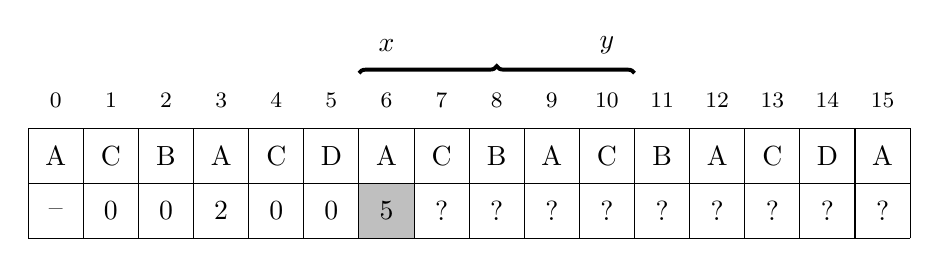
\begin{tikzpicture}[scale=0.7]
\fill[color=lightgray] (6,0) rectangle (7,1);
\draw (0,0) grid (16,2);

\node at (0.5, 1.5) {A};
\node at (1.5, 1.5) {C};
\node at (2.5, 1.5) {B};
\node at (3.5, 1.5) {A};
\node at (4.5, 1.5) {C};
\node at (5.5, 1.5) {D};
\node at (6.5, 1.5) {A};
\node at (7.5, 1.5) {C};
\node at (8.5, 1.5) {B};
\node at (9.5, 1.5) {A};
\node at (10.5, 1.5) {C};
\node at (11.5, 1.5) {B};
\node at (12.5, 1.5) {A};
\node at (13.5, 1.5) {C};
\node at (14.5, 1.5) {D};
\node at (15.5, 1.5) {A};

\node at (0.5, 0.5) {--};
\node at (1.5, 0.5) {0};
\node at (2.5, 0.5) {0};
\node at (3.5, 0.5) {2};
\node at (4.5, 0.5) {0};
\node at (5.5, 0.5) {0};
\node at (6.5, 0.5) {5};
\node at (7.5, 0.5) {?};
\node at (8.5, 0.5) {?};
\node at (9.5, 0.5) {?};
\node at (10.5, 0.5) {?};
\node at (11.5, 0.5) {?};
\node at (12.5, 0.5) {?};
\node at (13.5, 0.5) {?};
\node at (14.5, 0.5) {?};
\node at (15.5, 0.5) {?};

\draw [decoration={brace}, decorate, line width=0.5mm] (6,3.00) -- (11,3.00);

\node at (6.5,3.50) {$x$};
\node at (10.5,3.50) {$y$};


\footnotesize
\node at (0.5, 2.5) {0};
\node at (1.5, 2.5) {1};
\node at (2.5, 2.5) {2};
\node at (3.5, 2.5) {3};
\node at (4.5, 2.5) {4};
\node at (5.5, 2.5) {5};
\node at (6.5, 2.5) {6};
\node at (7.5, 2.5) {7};
\node at (8.5, 2.5) {8};
\node at (9.5, 2.5) {9};
\node at (10.5, 2.5) {10};
\node at (11.5, 2.5) {11};
\node at (12.5, 2.5) {12};
\node at (13.5, 2.5) {13};
\node at (14.5, 2.5) {14};
\node at (15.5, 2.5) {15};

\end{tikzpicture}
\end{center}

Sada možemo izračunati
sljedeće vrijednosti Z-niza
efikasno,
jer znamo da su
$\texttt{s}[0 \ldots 4]$ i
$\texttt{s}[6 \ldots 10]$ jednaki.
Prvo, budući da je $\texttt{z}[1] = \texttt{z}[2] = 0$,
odmah znamo da je i
$\texttt{z}[7] = \texttt{z}[8] = 0$:

\begin{center}
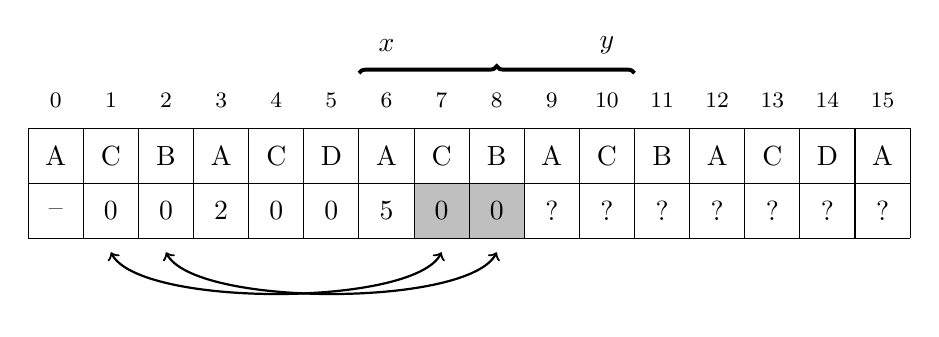
\begin{tikzpicture}[scale=0.7]
\fill[color=lightgray] (7,0) rectangle (9,1);
\draw (0,0) grid (16,2);

\node at (0.5, 1.5) {A};
\node at (1.5, 1.5) {C};
\node at (2.5, 1.5) {B};
\node at (3.5, 1.5) {A};
\node at (4.5, 1.5) {C};
\node at (5.5, 1.5) {D};
\node at (6.5, 1.5) {A};
\node at (7.5, 1.5) {C};
\node at (8.5, 1.5) {B};
\node at (9.5, 1.5) {A};
\node at (10.5, 1.5) {C};
\node at (11.5, 1.5) {B};
\node at (12.5, 1.5) {A};
\node at (13.5, 1.5) {C};
\node at (14.5, 1.5) {D};
\node at (15.5, 1.5) {A};

\node at (0.5, 0.5) {--};
\node at (1.5, 0.5) {0};
\node at (2.5, 0.5) {0};
\node at (3.5, 0.5) {2};
\node at (4.5, 0.5) {0};
\node at (5.5, 0.5) {0};
\node at (6.5, 0.5) {5};
\node at (7.5, 0.5) {0};
\node at (8.5, 0.5) {0};
\node at (9.5, 0.5) {?};
\node at (10.5, 0.5) {?};
\node at (11.5, 0.5) {?};
\node at (12.5, 0.5) {?};
\node at (13.5, 0.5) {?};
\node at (14.5, 0.5) {?};
\node at (15.5, 0.5) {?};


\draw [decoration={brace}, decorate, line width=0.5mm] (6,3.00) -- (11,3.00);

\node at (6.5,3.50) {$x$};
\node at (10.5,3.50) {$y$};


\footnotesize
\node at (0.5, 2.5) {0};
\node at (1.5, 2.5) {1};
\node at (2.5, 2.5) {2};
\node at (3.5, 2.5) {3};
\node at (4.5, 2.5) {4};
\node at (5.5, 2.5) {5};
\node at (6.5, 2.5) {6};
\node at (7.5, 2.5) {7};
\node at (8.5, 2.5) {8};
\node at (9.5, 2.5) {9};
\node at (10.5, 2.5) {10};
\node at (11.5, 2.5) {11};
\node at (12.5, 2.5) {12};
\node at (13.5, 2.5) {13};
\node at (14.5, 2.5) {14};
\node at (15.5, 2.5) {15};


\draw[thick,<->] (7.5,-0.25) .. controls (7,-1.25) and (2,-1.25) .. (1.5,-0.25);
\draw[thick,<->] (8.5,-0.25) .. controls (8,-1.25) and (3,-1.25) .. (2.5,-0.25);
\end{tikzpicture}
\end{center}

Zatim, budući da je $\texttt{z}[3]=2$, znamo da je $\texttt{z}[9] \ge 2$:

\begin{center}
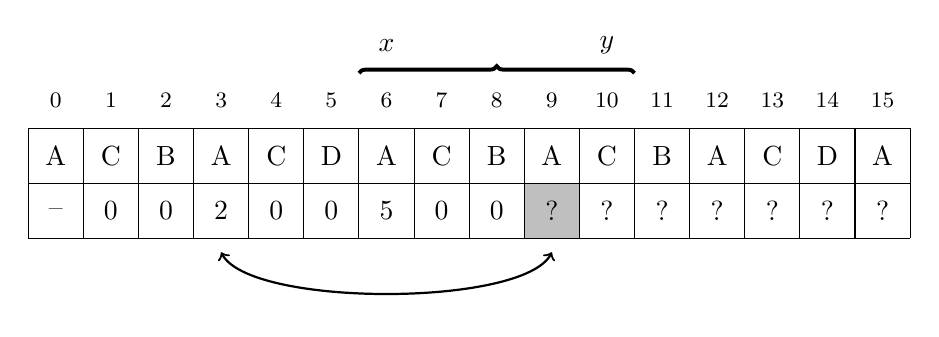
\begin{tikzpicture}[scale=0.7]
\fill[color=lightgray] (9,0) rectangle (10,1);
\draw (0,0) grid (16,2);

\node at (0.5, 1.5) {A};
\node at (1.5, 1.5) {C};
\node at (2.5, 1.5) {B};
\node at (3.5, 1.5) {A};
\node at (4.5, 1.5) {C};
\node at (5.5, 1.5) {D};
\node at (6.5, 1.5) {A};
\node at (7.5, 1.5) {C};
\node at (8.5, 1.5) {B};
\node at (9.5, 1.5) {A};
\node at (10.5, 1.5) {C};
\node at (11.5, 1.5) {B};
\node at (12.5, 1.5) {A};
\node at (13.5, 1.5) {C};
\node at (14.5, 1.5) {D};
\node at (15.5, 1.5) {A};

\node at (0.5, 0.5) {--};
\node at (1.5, 0.5) {0};
\node at (2.5, 0.5) {0};
\node at (3.5, 0.5) {2};
\node at (4.5, 0.5) {0};
\node at (5.5, 0.5) {0};
\node at (6.5, 0.5) {5};
\node at (7.5, 0.5) {0};
\node at (8.5, 0.5) {0};
\node at (9.5, 0.5) {?};
\node at (10.5, 0.5) {?};
\node at (11.5, 0.5) {?};
\node at (12.5, 0.5) {?};
\node at (13.5, 0.5) {?};
\node at (14.5, 0.5) {?};
\node at (15.5, 0.5) {?};

\draw [decoration={brace}, decorate, line width=0.5mm] (6,3.00) -- (11,3.00);

\node at (6.5,3.50) {$x$};
\node at (10.5,3.50) {$y$};


\footnotesize
\node at (0.5, 2.5) {0};
\node at (1.5, 2.5) {1};
\node at (2.5, 2.5) {2};
\node at (3.5, 2.5) {3};
\node at (4.5, 2.5) {4};
\node at (5.5, 2.5) {5};
\node at (6.5, 2.5) {6};
\node at (7.5, 2.5) {7};
\node at (8.5, 2.5) {8};
\node at (9.5, 2.5) {9};
\node at (10.5, 2.5) {10};
\node at (11.5, 2.5) {11};
\node at (12.5, 2.5) {12};
\node at (13.5, 2.5) {13};
\node at (14.5, 2.5) {14};
\node at (15.5, 2.5) {15};

\draw[thick,<->] (9.5,-0.25) .. controls (9,-1.25) and (4,-1.25) .. (3.5,-0.25);
\end{tikzpicture}
\end{center}

Međutim, o znakovnom nizu nakon pozicije 10
nemamo nikakvih informacija, pa moramo usporediti podnizove
znakova znak po znak:

\begin{center}
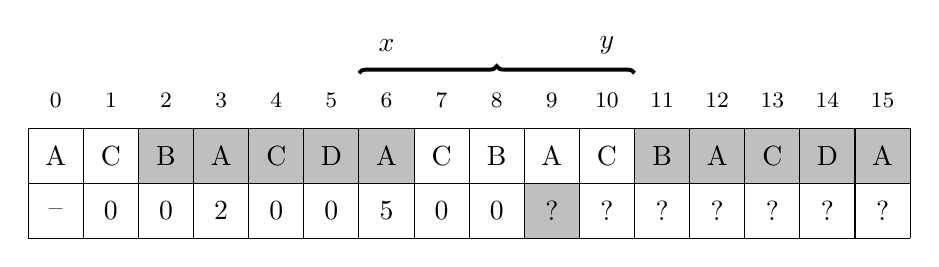
\begin{tikzpicture}[scale=0.7]
\fill[color=lightgray] (9,0) rectangle (10,1);
\fill[color=lightgray] (2,1) rectangle (7,2);
\fill[color=lightgray] (11,1) rectangle (16,2);


\draw (0,0) grid (16,2);

\node at (0.5, 1.5) {A};
\node at (1.5, 1.5) {C};
\node at (2.5, 1.5) {B};
\node at (3.5, 1.5) {A};
\node at (4.5, 1.5) {C};
\node at (5.5, 1.5) {D};
\node at (6.5, 1.5) {A};
\node at (7.5, 1.5) {C};
\node at (8.5, 1.5) {B};
\node at (9.5, 1.5) {A};
\node at (10.5, 1.5) {C};
\node at (11.5, 1.5) {B};
\node at (12.5, 1.5) {A};
\node at (13.5, 1.5) {C};
\node at (14.5, 1.5) {D};
\node at (15.5, 1.5) {A};

\node at (0.5, 0.5) {--};
\node at (1.5, 0.5) {0};
\node at (2.5, 0.5) {0};
\node at (3.5, 0.5) {2};
\node at (4.5, 0.5) {0};
\node at (5.5, 0.5) {0};
\node at (6.5, 0.5) {5};
\node at (7.5, 0.5) {0};
\node at (8.5, 0.5) {0};
\node at (9.5, 0.5) {?};
\node at (10.5, 0.5) {?};
\node at (11.5, 0.5) {?};
\node at (12.5, 0.5) {?};
\node at (13.5, 0.5) {?};
\node at (14.5, 0.5) {?};
\node at (15.5, 0.5) {?};

\draw [decoration={brace}, decorate, line width=0.5mm] (6,3.00) -- (11,3.00);

\node at (6.5,3.50) {$x$};
\node at (10.5,3.50) {$y$};


\footnotesize
\node at (0.5, 2.5) {0};
\node at (1.5, 2.5) {1};
\node at (2.5, 2.5) {2};
\node at (3.5, 2.5) {3};
\node at (4.5, 2.5) {4};
\node at (5.5, 2.5) {5};
\node at (6.5, 2.5) {6};
\node at (7.5, 2.5) {7};
\node at (8.5, 2.5) {8};
\node at (9.5, 2.5) {9};
\node at (10.5, 2.5) {10};
\node at (11.5, 2.5) {11};
\node at (12.5, 2.5) {12};
\node at (13.5, 2.5) {13};
\node at (14.5, 2.5) {14};
\node at (15.5, 2.5) {15};

%\draw[thick,<->] (11.5,-0.25) .. controls (11,-1.25) and (3,-1.25) .. (2.5,-0.25);
\end{tikzpicture}
\end{center}

Pokazuje se da je $\texttt{z}[9]=7$,
pa je novi interval $[x,y]$ jednak $[9,15]$:

\begin{center}
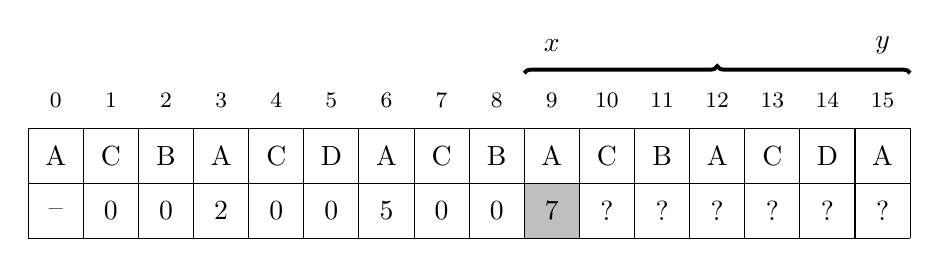
\begin{tikzpicture}[scale=0.7]
\fill[color=lightgray] (9,0) rectangle (10,1);
\draw (0,0) grid (16,2);

\node at (0.5, 1.5) {A};
\node at (1.5, 1.5) {C};
\node at (2.5, 1.5) {B};
\node at (3.5, 1.5) {A};
\node at (4.5, 1.5) {C};
\node at (5.5, 1.5) {D};
\node at (6.5, 1.5) {A};
\node at (7.5, 1.5) {C};
\node at (8.5, 1.5) {B};
\node at (9.5, 1.5) {A};
\node at (10.5, 1.5) {C};
\node at (11.5, 1.5) {B};
\node at (12.5, 1.5) {A};
\node at (13.5, 1.5) {C};
\node at (14.5, 1.5) {D};
\node at (15.5, 1.5) {A};

\node at (0.5, 0.5) {--};
\node at (1.5, 0.5) {0};
\node at (2.5, 0.5) {0};
\node at (3.5, 0.5) {2};
\node at (4.5, 0.5) {0};
\node at (5.5, 0.5) {0};
\node at (6.5, 0.5) {5};
\node at (7.5, 0.5) {0};
\node at (8.5, 0.5) {0};
\node at (9.5, 0.5) {7};
\node at (10.5, 0.5) {?};
\node at (11.5, 0.5) {?};
\node at (12.5, 0.5) {?};
\node at (13.5, 0.5) {?};
\node at (14.5, 0.5) {?};
\node at (15.5, 0.5) {?};

\draw [decoration={brace}, decorate, line width=0.5mm] (9,3.00) -- (16,3.00);

\node at (9.5,3.50) {$x$};
\node at (15.5,3.50) {$y$};


\footnotesize
\node at (0.5, 2.5) {0};
\node at (1.5, 2.5) {1};
\node at (2.5, 2.5) {2};
\node at (3.5, 2.5) {3};
\node at (4.5, 2.5) {4};
\node at (5.5, 2.5) {5};
\node at (6.5, 2.5) {6};
\node at (7.5, 2.5) {7};
\node at (8.5, 2.5) {8};
\node at (9.5, 2.5) {9};
\node at (10.5, 2.5) {10};
\node at (11.5, 2.5) {11};
\node at (12.5, 2.5) {12};
\node at (13.5, 2.5) {13};
\node at (14.5, 2.5) {14};
\node at (15.5, 2.5) {15};

% \draw[thick,<->] (9.5,-0.25) .. controls (9,-1.25) and (4,-1.25) .. (3.5,-0.25);
\end{tikzpicture}
\end{center}

Nakon toga sve ostale vrijednosti Z-niza
možemo odrediti koristeći informacije
koje su već pohranjene u Z-nizu:

\begin{center}
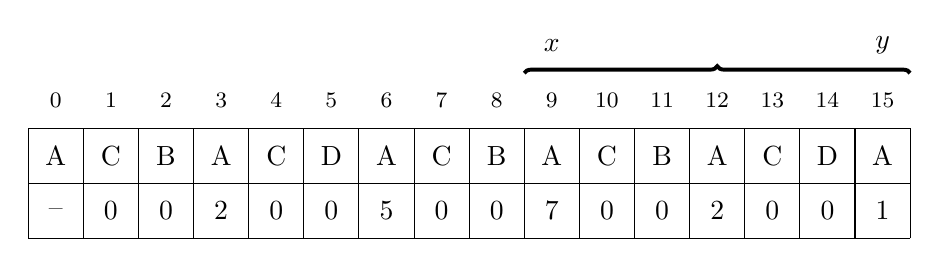
\begin{tikzpicture}[scale=0.7]
\draw (0,0) grid (16,2);

\node at (0.5, 1.5) {A};
\node at (1.5, 1.5) {C};
\node at (2.5, 1.5) {B};
\node at (3.5, 1.5) {A};
\node at (4.5, 1.5) {C};
\node at (5.5, 1.5) {D};
\node at (6.5, 1.5) {A};
\node at (7.5, 1.5) {C};
\node at (8.5, 1.5) {B};
\node at (9.5, 1.5) {A};
\node at (10.5, 1.5) {C};
\node at (11.5, 1.5) {B};
\node at (12.5, 1.5) {A};
\node at (13.5, 1.5) {C};
\node at (14.5, 1.5) {D};
\node at (15.5, 1.5) {A};

\node at (0.5, 0.5) {--};
\node at (1.5, 0.5) {0};
\node at (2.5, 0.5) {0};
\node at (3.5, 0.5) {2};
\node at (4.5, 0.5) {0};
\node at (5.5, 0.5) {0};
\node at (6.5, 0.5) {5};
\node at (7.5, 0.5) {0};
\node at (8.5, 0.5) {0};
\node at (9.5, 0.5) {7};
\node at (10.5, 0.5) {0};
\node at (11.5, 0.5) {0};
\node at (12.5, 0.5) {2};
\node at (13.5, 0.5) {0};
\node at (14.5, 0.5) {0};
\node at (15.5, 0.5) {1};

\draw [decoration={brace}, decorate, line width=0.5mm] (9,3.00) -- (16,3.00);

\node at (9.5,3.50) {$x$};
\node at (15.5,3.50) {$y$};


\footnotesize
\node at (0.5, 2.5) {0};
\node at (1.5, 2.5) {1};
\node at (2.5, 2.5) {2};
\node at (3.5, 2.5) {3};
\node at (4.5, 2.5) {4};
\node at (5.5, 2.5) {5};
\node at (6.5, 2.5) {6};
\node at (7.5, 2.5) {7};
\node at (8.5, 2.5) {8};
\node at (9.5, 2.5) {9};
\node at (10.5, 2.5) {10};
\node at (11.5, 2.5) {11};
\node at (12.5, 2.5) {12};
\node at (13.5, 2.5) {13};
\node at (14.5, 2.5) {14};
\node at (15.5, 2.5) {15};

\end{tikzpicture}
\end{center}

\subsubsection{Uporaba Z-niza}

Često je stvar ukusa hoćemo li koristiti
raspršivanje znakovnih nizova ili Z-algoritam.
Za razliku od raspršivanja, Z-algoritam uvijek radi
i nema opasnosti od kolizija.
S druge strane, Z-algoritam je teže
implementirati, a neki se zadaci mogu riješiti
samo raspršivanjem.

Kao primjer razmotrimo ponovno
zadatak traženja uzorka,
gdje je naš zadatak naći pojave
uzorka $p$ u znakovnom nizu $s$.
Taj smo zadatak već efikasno riješili
raspršivanjem znakovnih nizova, no Z-algoritam
nudi drugi način rješavanja zadatka.

Uobičajena ideja u obradi znakovnih nizova je
konstruirati znakovni niz koji se sastoji od
više nizova razdvojenih specijalnim znakovima.
U ovom zadatku možemo konstruirati znakovni niz
$p$\texttt{\#}$s$,
gdje su $p$ i $s$ razdvojeni specijalnim
znakom \texttt{\#} koji se ne pojavljuje
u tim nizovima.
Z-niz niza $p$\texttt{\#}$s$ govori nam pozicije
na kojima se $p$ pojavljuje u $s$,
jer takve pozicije sadrže duljinu niza $p$.

Na primjer, ako je $s=$\texttt{HATTIVATTI} i $p=$\texttt{ATT},
Z-niz je sljedeći:

\begin{center}
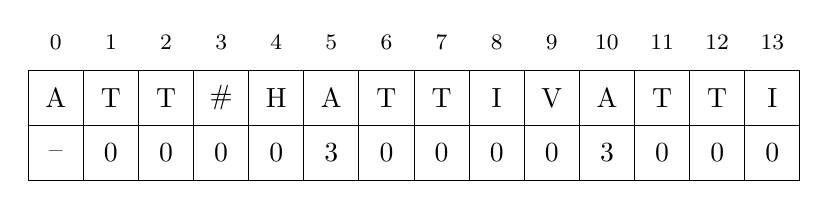
\begin{tikzpicture}[scale=0.7]
\draw (0,0) grid (14,2);

\node at (0.5, 1.5) {A};
\node at (1.5, 1.5) {T};
\node at (2.5, 1.5) {T};
\node at (3.5, 1.5) {\#};
\node at (4.5, 1.5) {H};
\node at (5.5, 1.5) {A};
\node at (6.5, 1.5) {T};
\node at (7.5, 1.5) {T};
\node at (8.5, 1.5) {I};
\node at (9.5, 1.5) {V};
\node at (10.5, 1.5) {A};
\node at (11.5, 1.5) {T};
\node at (12.5, 1.5) {T};
\node at (13.5, 1.5) {I};

\node at (0.5, 0.5) {--};
\node at (1.5, 0.5) {0};
\node at (2.5, 0.5) {0};
\node at (3.5, 0.5) {0};
\node at (4.5, 0.5) {0};
\node at (5.5, 0.5) {3};
\node at (6.5, 0.5) {0};
\node at (7.5, 0.5) {0};
\node at (8.5, 0.5) {0};
\node at (9.5, 0.5) {0};
\node at (10.5, 0.5) {3};
\node at (11.5, 0.5) {0};
\node at (12.5, 0.5) {0};
\node at (13.5, 0.5) {0};

\footnotesize
\node at (0.5, 2.5) {0};
\node at (1.5, 2.5) {1};
\node at (2.5, 2.5) {2};
\node at (3.5, 2.5) {3};
\node at (4.5, 2.5) {4};
\node at (5.5, 2.5) {5};
\node at (6.5, 2.5) {6};
\node at (7.5, 2.5) {7};
\node at (8.5, 2.5) {8};
\node at (9.5, 2.5) {9};
\node at (10.5, 2.5) {10};
\node at (11.5, 2.5) {11};
\node at (12.5, 2.5) {12};
\node at (13.5, 2.5) {13};
\end{tikzpicture}
\end{center}

Pozicije 5 i 10 sadrže vrijednost 3,
što znači da se uzorak \texttt{ATT}
pojavljuje na odgovarajućim pozicijama
niza \texttt{HATTIVATTI}.

Vremenska složenost dobivenog algoritma
linearna je, jer je dovoljno konstruirati
Z-niz i proći kroz njegove vrijednosti.

\subsubsection{Implementacija}

Slijedi kratka implementacija Z-algoritma
koja vraća vektor koji odgovara Z-nizu.

\begin{lstlisting}
vector<int> z(string s) {
    int n = s.size();
    vector<int> z(n);
    int x = 0, y = 0;
    for (int i = 1; i < n; i++) {
        z[i] = max(0,min(z[i-x],y-i+1));
        while (i+z[i] < n && s[z[i]] == s[i+z[i]]) {
            x = i; y = i+z[i]; z[i]++;
        }
    }
    return z;
}
\end{lstlisting}